\section{Experiment 10H-J: bound sensitivity and single-model validation}
\label{sec:experiment10hj}

\paragraph{Purpose and status of the bounds.}
Experiments 10H-H/I produced repeatable constrained optima but left active
bounds, shallow profiles and miscalibrated innovations. The inherited
coefficient multipliers 0.35 and 3 were introduced in 10H-G without a
documented engineering-range derivation. Their preservation made the earlier
comparisons controlled; it did not make them calibrated physical limits.
Physical coupling and positive coordinates establish realizability in the
adopted bicycle structure, not plausibility for the intended vehicle envelope.

For a uniform coefficient box with nominal multipliers $a,b$, axle distances
and normalized stiffnesses have marginal relative ranges $[a/b,b/a]$;
$m/I_z$ has range $[a^2/b,b^2/a]$. Relaxation lengths and the actuator time
constant have relative ranges $[1/b,1/a]$. Thus the original box permits a
nominal 2.8\,m wheelbase to range from 0.327 to 24\,m even under exact coupling.
These marginal intervals are not independent physical prior boxes.
The provenance and required engineering evidence are recorded in
\texttt{docs/experiment\_10hj\_bound\_provenance.md}. Public model definitions
support the quantities but do not justify fleet-wide numerical ranges
\cite{mathworksVehicleBody2026}.

\paragraph{Predeclared diagnostic.}
Before execution, commit \texttt{aadfc7f} fixes three nested coefficient boxes,
$[0.35,3]$, $[0.2,5]$, and $[0.1,10]$, in two separate fixed-$Q$ panels at
scales 0.01 and 1. All boxes retain eight positive coordinates and exact
coupling. The same opened fleets 601--605, measured records, 200-sample
segments and training/held-out client positions are used. Array hashes must
match 10H-I before fitting. The 0.01 panel is a historical controlled setting;
it is not a newly validated covariance-selection rule. Neither a bound nor a
covariance setting is selected in this study. Three deterministic staged
starts use 80 iterations per restricted stage and 500 for joint refinement;
only training working likelihood selects a restart. Confirmation seeds
591--600 and 611--620 remain sealed.

The numerical audit checks independent KKT residuals, feasibility, gradients,
coupling, restart consistency, full/active-face curvature, and monotonic best
training likelihood under nested feasible sets. Every widest-box model has
eight nuisance-reoptimized profiles at offsets $0,\pm0.08,\pm0.16$. A separate
profile fixes $b_r/b_{r,\mathrm{nom}}$ at
$0.1,0.15,0.2,0.25,0.35,0.5,1$ and reoptimizes the seven other coordinates.
Infeasible targets are recorded. Working-objective profiles are not calibrated
confidence intervals for this heterogeneous model.

\paragraph{Causal output validation.}
All predeclared models are scored after training selection. Forecast horizons
are 1, 5, 20 and 50 samples, or 0.01, 0.05, 0.2 and 0.5\,s. With a
20-sample observation burn-in, each horizon uses identical forecast origins.
The filtered state uses outputs strictly before its origin; subsequent
propagation uses known commands with no intervening output corrections.
Zero-initialized full-record simulation is a separate diagnostic. This
separates measurement-assisted one-step prediction from longer-horizon
dynamic validation \cite{mathworksPrediction2026}.

Innovation covariance, normalized NIS, means, and correlations at lags 1--20
are also reported. Positive lags pair the present innovation with past
innovations or past steering commands, without crossing record boundaries.
Pooled and within-record-centered correlations expose sensitivity to constant
bias. They are descriptive; no independent-sample significance threshold is
applied to heterogeneous, temporally dependent records. Residual--input
correlation complements residual whiteness in model validation
\cite{mathworksResidual2026}.

\paragraph{Interpretation.}
The wider boxes are diagnostic domains, not proposed engineering priors.
No new zero-active-bound acceptance gate is introduced, and historical gate
results remain unchanged. An interior solution alone does not establish
physical calibration; an active bound alone does not invalidate a constrained
optimum. Persistent boundary motion or weak profiles indicates unresolved
sensitivity, but cannot isolate fleet heterogeneity from covariance or bias
mismatch. No latent-state accuracy or closed-loop-control gain is claimed.

\paragraph{Numerical result.}
All 90 model restarts satisfy the declared independent KKT and feasibility
checks, with maximum stationarity residual $1.17\times10^{-5}$, maximum
parameter CV $2.83\times10^{-6}$ and coupling error
$1.78\times10^{-15}$. No fitting evaluation is invalid. Every nested best
training objective is nonincreasing. All feasible local and extended
rear-gain profiles also satisfy stationarity and feasibility checks.
The original-box fits reproduce the 10H-I staged objectives and held-out
errors. Table~\ref{tab:10hj-boxes} reports the complete predeclared comparison.

\begin{table}[htbp]
\centering
\caption{Mean full-record held-out one-step fixed-$R$ error and fleets with
active coefficient bounds. All five fleets are included in each row.}
\label{tab:10hj-boxes}
\begin{tabular}{llrr}
\toprule
$Q$ scale & Coefficient multipliers & Mean $E_R$ & Boundary fleets\\
\midrule
0.01 & $[0.35,3]$ & 5.010 & 5/5\\
0.01 & $[0.2,5]$ & 4.729 & 5/5\\
0.01 & $[0.1,10]$ & 4.126 & 5/5\\
1 & $[0.35,3]$ & 1.996 & 5/5\\
1 & $[0.2,5]$ & 1.955 & 3/5\\
1 & $[0.1,10]$ & 1.945 & 1/5\\
\bottomrule
\end{tabular}
\end{table}

At scale 0.01, every rear gain follows the changing floor exactly:
$b_r/b_{r,\mathrm{nom}}=0.35,0.2,0.1$. The widest-box gain is
9.596\,s$^{-2}$ throughout. Rear axle distances move to 2.558--2.913\,m and
normalized rear stiffnesses change with the bound. The mean paired one-step
error reduction is 17.55\%, with range 14.46--19.77\%, but an interior physical
calibration has not emerged. Outward profiles remain infeasible at the new
rear-gain floor. Correct KKT signs and positive face curvature establish
valid constrained optima, not that the floor has a physical justification.

At scale 1, four widest-box models are interior; seed 604 still hits the
rear-gain floor. Seeds 601 and 603 already settle in the middle box, and
further widening preserves their optima. The widest rear gains range from
9.596 to 21.401\,s$^{-2}$, rear axle distances from 2.174 to 2.909\,m and rear
relaxation lengths from 1.754 to 3.020\,m. These are fitted working-model
quantities, not comparisons with true client parameters. Mean paired one-step
error reduction versus the original box is 2.54\% (1.18--3.97\%).
Weak profiles remain: the smallest feasible local profile-edge increase is
0.00194\% of working likelihood. For seed 605 the negative force-gain offset
$-0.16$ is infeasible even though the fit is interior; its negative profile
edge is $-0.08$. Thus interiority does not imply adequate distance from the
limit or useful calibrated uncertainty.

\paragraph{Longer-horizon result.}
Table~\ref{tab:10hj-forecasts} uses the identical 131 origins per record at
all forecast horizons. Its one-step values differ from full-record scores
because burn-in and common-origin truncation change the scoring window.
The full simulation uses all 200 samples and no output corrections.

\begin{table}[htbp]
\centering
\caption{Mean fixed-$R$ output error for causal forecasts and full-record
simulation. Nominal simulation is independent of $Q$; filtered initialization
makes nominal finite-horizon forecasts depend on $Q$.}
\label{tab:10hj-forecasts}
\begin{tabular}{llrrrr}
\toprule
$Q$ scale & Model/box & 1 step & 20 steps & 50 steps & Simulation\\
\midrule
0.01 & Original & 4.909 & 98.069 & 178.614 & 167.904\\
0.01 & Widest & 3.962 & 98.657 & 164.766 & 156.155\\
1 & Original & 1.968 & 88.571 & 170.535 & 170.155\\
1 & Wider & 1.921 & 92.264 & 192.734 & 203.233\\
1 & Widest & 1.907 & 98.289 & 222.477 & 236.497\\
1 & Nominal & 2.171 & 93.114 & 160.011 & 150.066\\
\bottomrule
\end{tabular}
\end{table}

At scale 0.01, widening improves the 50-step error in all five fleets, with
mean paired reduction 7.99\%, but the widest model is worse than the nominal
model in four fleets at that horizon and in four under simulation. At scale
1, the widest model improves one-step and five-step prediction, while
50-step error worsens in every fleet versus the original box. Mean paired
50-step degradation is 29.82\% (7.57--58.88\%); four fleets also perform worse
than nominal at that horizon. Full simulation deteriorates in all five
fleets versus both the original box and the nominal model. These are output
dynamics checks, not latent-state or closed-loop-control tests.

\begin{figure}[htbp]
\centering
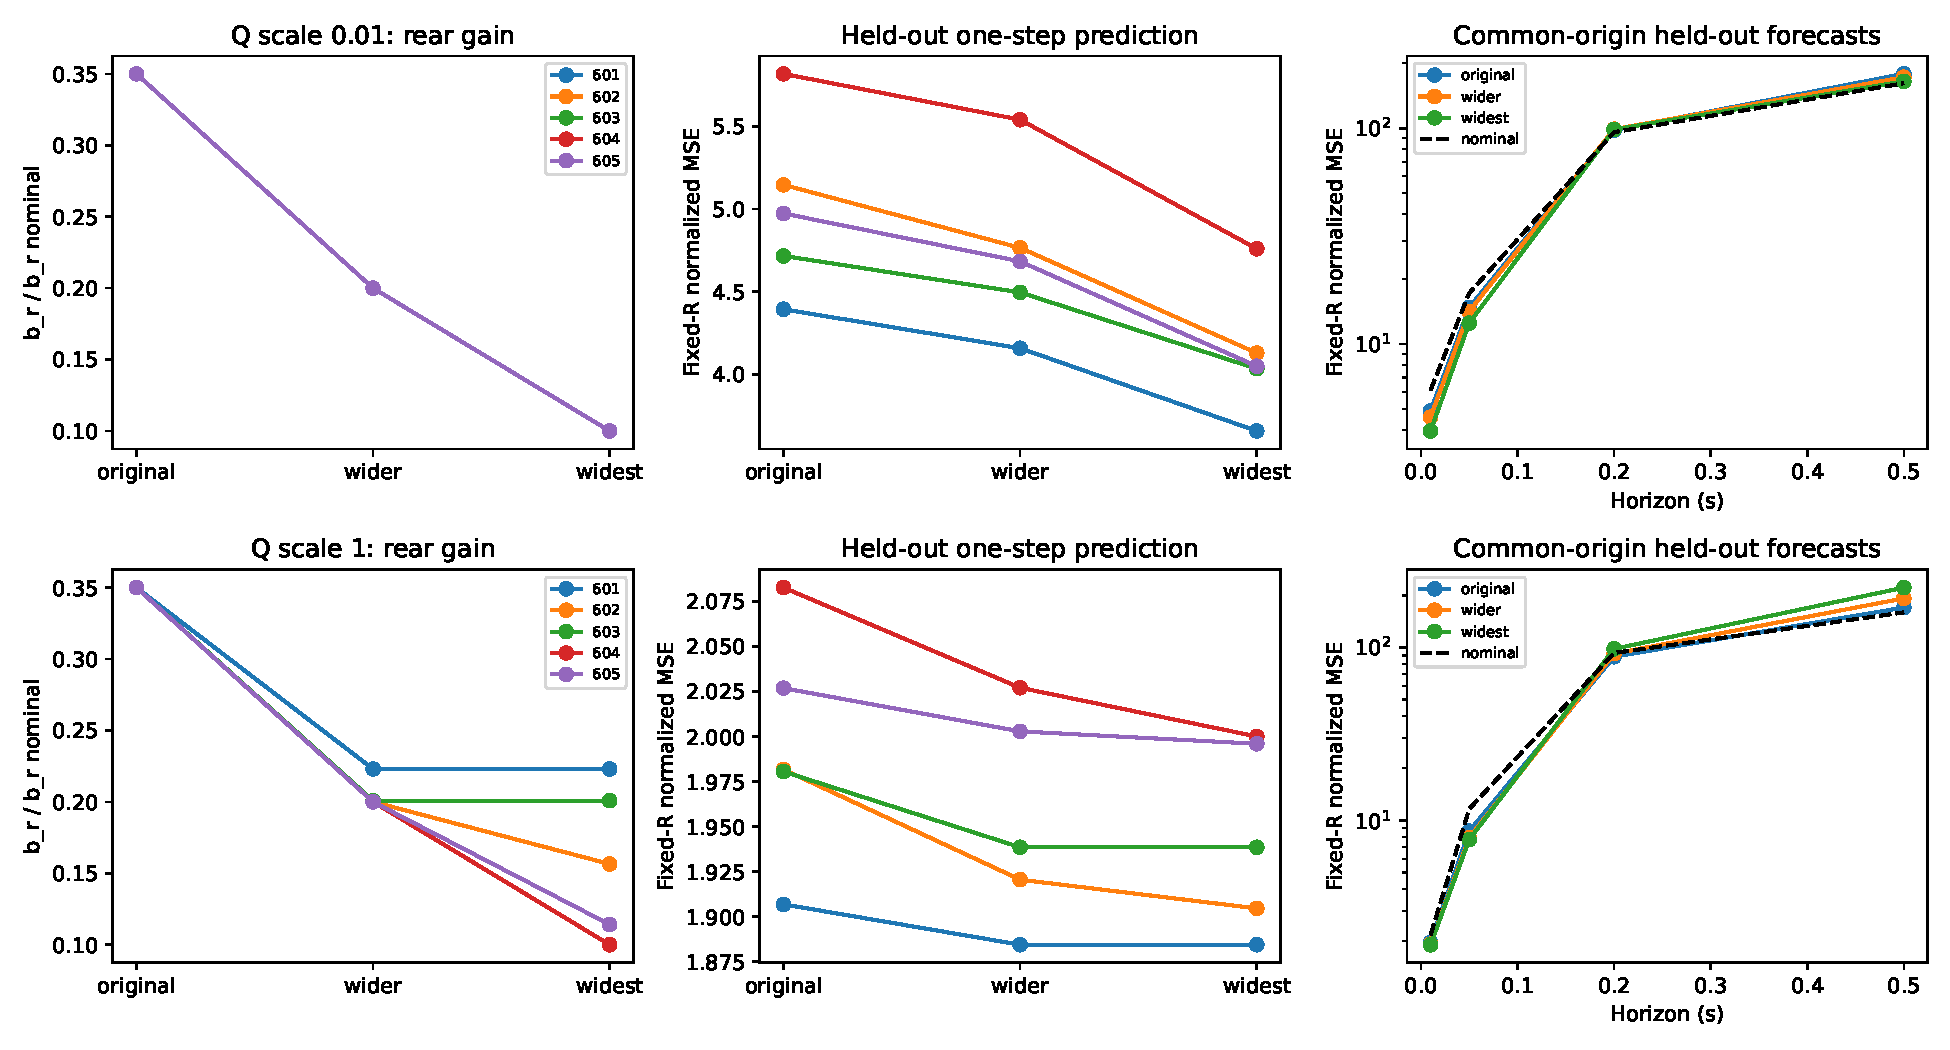
\includegraphics[width=\linewidth]{../results/figures/experiment_10hj_bound_sensitivity.pdf}
\caption{Rear-gain boundary motion, one-step errors and common-origin
forecast errors. The curves expose covariance-dependent boundary behavior
and the difference between short-horizon prediction and dynamic validation.}
\end{figure}

\paragraph{Residual calibration and scientific decision.}
For widest-box models, mean normalized NIS is 3.285 at scale 0.01 and 0.437
at scale 1, rather than the correctly specified Gaussian reference of one.
Maximum within-record innovation autocorrelation over lags 1--20 is 0.812
and 0.347, respectively; maximum correlation with past commands is 0.322 and
0.173. Scale-1 whitened covariance eigenvalues remain below one, with minimum
eigenvalues 0.174--0.184 and maximum eigenvalues 0.694--0.731. Removing record
means does not eliminate the serial correlation. Every fitted model is stable
at the measured scheduling speeds (maximum discrete plant spectral radius
0.994), so forecast degradation is not explained by an unstable fitted pole
at these speeds. This finite-speed check is not a continuous-speed stability
certificate.

The diagnostic answers the bound question: the original box was restrictive
for some optima, but expanding it is insufficient to establish a calibrated
physical model. Numerical repair is successful. The scientific bottleneck
is now prediction-focus, pooled-model mismatch and uncertainty calibration.
No widest box is adopted as an engineering prior and no historical gate is
reclassified. Actual physical intervals require independent evidence for a
defined vehicle envelope, using the transformed geometry, normalized
stiffness, relaxation and actuator quantities.

The next bounded study should compare label-blind $K=1$ and $K=2$ jointly
learned models under common covariance/bias assumptions, with client-blocked
training selection and predeclared multi-step and simulation validation.
A one-step working-likelihood gain alone must not establish improved dynamics
or calibrated grouping probabilities. This comparison should test whether
multiple compatible models resolve the observed mismatch; it should not
require the heterogeneous $K=1$ model to become physically perfect first.

\paragraph{Reproducibility.}
The configuration and numerical source were committed before execution.
A subsequent reporting-only correction fixes access to the forecast
\texttt{mode} column in the figure. All ten execution manifests retain
commit \texttt{aadfc7f}, archived source fingerprints and output hashes.
Summary reconstruction verifies that all fitting code and other execution
sources are unchanged before accepting this reporting update. No fit,
profile, bound, covariance, data split or numerical criterion is changed.
Independent tests cover forecast timing, absence of future-output leakage,
known-model recovery, one-step scoring equivalence and record boundaries.
The full suite passes 130 tests; lint passes for the new Python files.
